\section{Produktfunktionen}

\subsection{Use case - Anschauen der Gästebucheinträge}

\begin{figurehere}
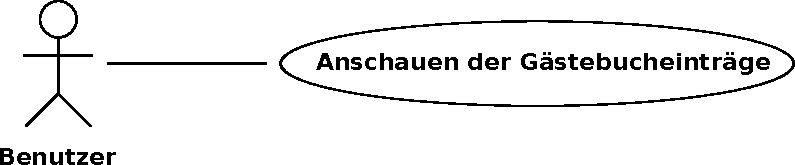
\includegraphics[width=\columnwidth]{use-case-show_entries}
\captionof{figure}{Anschauen der Gästebucheinträge}
\end{figurehere}

\paragraph{Ziel des Use Cases:}

\begin{asparaitem}
\item Ein Benutzer kann die Gästebucheinträge sehen.
\end{asparaitem}


\paragraph{Umgebende Systemgrenze:}

Die Gästebuch-Web-App.

\paragraph{Vorbedingung:}

Das Gästebuch-App ist auf dem System installiert und konfiguriert.

\paragraph{Nachbedingung bei erfolgreicher Ausführung:}

\begin{asparaitem}
\item Die Seite die die Gästebucheinträge darstellt wird dem Benutzer präsentiert.
\end{asparaitem}

\paragraph{Beteiligte Nutzer:}

\begin{asparaitem}
\item Benutzer.
\end{asparaitem}

\paragraph{Auslösendes Ereignis:}

\begin{asparaitem}
\item Der Benutzer besucht die Seite \url{http://gaestebuch/}
\end{asparaitem}

\subsection{Use case - Neuen Gästebucheintrag erstellen}

\begin{figurehere}
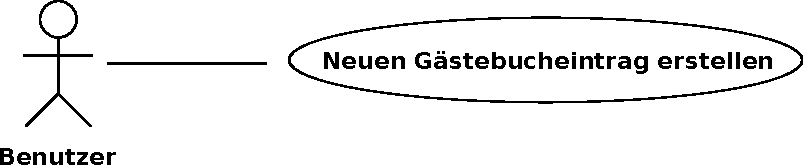
\includegraphics[width=\columnwidth]{use-case-new_entry}
\captionof{figure}{Neuen Gästebucheintrag erstellen}
\end{figurehere}

\paragraph{Ziel des Use Cases:}

\begin{asparaitem}
\item Ein Benutzer kann einen neuen Gästebucheintrag erstellen.
\end{asparaitem}

\paragraph{Umgebende Systemgrenze:}

Die Gästebuch-Web-App.

\paragraph{Vorbedingung:}

Das Gästebuch-App ist auf dem System installiert und konfiguriert.

\paragraph{Nachbedingung bei erfolgreicher Ausführung:}

\begin{asparaitem}
\item Ein neuer Gästebucheintrag ist im System erstellt.
\end{asparaitem}

\paragraph{Beteiligte Nutzer:}

\begin{asparaitem}
\item Benutzer.
\end{asparaitem}

\paragraph{Auslösendes Ereignis:}

\begin{asparaitem}
\item Der Benutzer besucht klickt auf den Button ``New Entry''.
\end{asparaitem}

